\iffalse
\documentclass[journal,12pt,twocolumn]{IEEEtran}
%
\usepackage{setspace}
\usepackage{gensymb}
%\doublespacing
\singlespacing

%\usepackage{graphicx}
%\usepackage{amssymb}
%\usepackage{relsize}
\usepackage[cmex10]{amsmath}
\usepackage{siunitx}
%\usepackage{amsthm}
%\interdisplaylinepenalty=2500
%\savesymbol{iint}
%\usepackage{txfonts}
%\restoresymbol{TXF}{iint}
%\usepackage{wasysym}
\usepackage{amsthm}
%\usepackage{iithtlc}
\usepackage{mathrsfs}
\usepackage{txfonts}
\usepackage{stfloats}
\usepackage{steinmetz}
\usepackage{supertabular}
%\usepackage{bm}
\usepackage{cite}
\usepackage{cases}
\usepackage{subfig}
%\usepackage{xtab}
\usepackage{longtable}
\usepackage{multirow}
%\usepackage{algorithm}
%\usepackage{algpseudocode}
\usepackage{enumitem}
\usepackage{mathtools}
\usepackage{tikz}
\usepackage{circuitikz}
\usepackage{verbatim}
\usepackage{tfrupee}
\usepackage[breaklinks=true]{hyperref}
%\usepackage{stmaryrd}
\usepackage{tkz-euclide} % loads  TikZ and tkz-base
%\usetkzobj{all}
\usetikzlibrary{calc,math}
\usetikzlibrary{fadings}
\usepackage{listings}
    \usepackage{color}                                            %%
    \usepackage{array}                                            %%
    \usepackage{longtable}                                        %%
    \usepackage{calc}                                             %%
    \usepackage{multirow}                                         %%
    \usepackage{hhline}                                           %%
    \usepackage{ifthen}                                           %%
  %optionally (for landscape tables embedded in another document): %%
    \usepackage{lscape}     
\usepackage{multicol}
\usepackage{chngcntr}
\usepackage{blkarray}
\usepackage{karnaugh-map}
\usepackage{fontspec}
\usepackage[intoc]{nomencl}
\makenomenclature

%\usetikzlibrary{arrows, shapes.gates.logic.US, calc}
\usetikzlibrary{arrows,shapes.gates.logic.US,shapes.gates.logic.IEC,calc}
\setmainfont{Sanskrit_2003.ttf}
%\setmainfont{Nakula.ttf}
%\setmainfont{Lohit-Devanagari.ttf}


%\usepackage{enumerate}

%\usepackage{wasysym}
%\newcounter{MYtempeqncnt}
\DeclareMathOperator*{\Res}{Res}
%\renewcommand{\baselinestretch}{2}
\renewcommand\thesection{\arabic{section}}
\renewcommand\thesubsection{\thesection.\arabic{subsection}}
\renewcommand\thesubsubsection{\thesubsection.\arabic{subsubsection}}

\renewcommand\thesectiondis{\arabic{section}}
\renewcommand\thesubsectiondis{\thesectiondis.\arabic{subsection}}
\renewcommand\thesubsubsectiondis{\thesubsectiondis.\arabic{subsubsection}}

% correct bad hyphenation here
\hyphenation{op-tical net-works semi-conduc-tor}
\def\inputGnumericTable{}                                 %%


\lstset{
%language=shell,
%language = Prolog,
frame=single, 
breaklines=true,
%showstringspaces=false,
columns=fullflexible
literate = {-}{-}1
}
%\lstset{
%language=tex,
%frame=single, 
%breaklines=true
%}

\begin{document}
%


\newtheorem{theorem}{Theorem}[section]
\newtheorem{problem}{Problem}
\newtheorem{proposition}{Proposition}[section]
\newtheorem{lemma}{Lemma}[section]
\newtheorem{corollary}[theorem]{Corollary}
\newtheorem{example}{Example}[section]
\newtheorem{definition}[problem]{Definition}
%\newtheorem{thm}{Theorem}[section] 
%\newtheorem{defn}[thm]{Definition}
%\newtheorem{algorithm}{Algorithm}[section]
%\newtheorem{cor}{Corollary}
\newcommand{\BEQA}{\begin{eqnarray}}
\newcommand{\EEQA}{\end{eqnarray}}
\newcommand{\define}{\stackrel{\triangle}{=}}

\bibliographystyle{IEEEtran}
%\bibliographystyle{ieeetr}


\providecommand{\mbf}{\mathbf}
\providecommand{\pr}[1]{\ensuremath{\Pr\left(#1\right)}}
\providecommand{\qfunc}[1]{\ensuremath{Q\left(#1\right)}}
\providecommand{\sbrak}[1]{\ensuremath{{}\left[#1\right]}}
\providecommand{\lsbrak}[1]{\ensuremath{{}\left[#1\right.}}
\providecommand{\rsbrak}[1]{\ensuremath{{}\left.#1\right]}}
\providecommand{\brak}[1]{\ensuremath{\left(#1\right)}}
\providecommand{\lbrak}[1]{\ensuremath{\left(#1\right.}}
\providecommand{\rbrak}[1]{\ensuremath{\left.#1\right)}}
\providecommand{\cbrak}[1]{\ensuremath{\left\{#1\right\}}}
\providecommand{\lcbrak}[1]{\ensuremath{\left\{#1\right.}}
\providecommand{\rcbrak}[1]{\ensuremath{\left.#1\right\}}}
\providecommand{\ceil}[1]{\left \lceil #1 \right \rceil }
\theoremstyle{remark}
\newtheorem{rem}{Remark}
\newcommand{\sgn}{\mathop{\mathrm{sgn}}}
\providecommand{\abs}[1]{\left\vert#1\right\vert}
\providecommand{\res}[1]{\Res\displaylimits_{#1}} 
\providecommand{\norm}[1]{\left\lVert#1\right\rVert}
%\providecommand{\norm}[1]{\lVert#1\rVert}
\providecommand{\mtx}[1]{\mathbf{#1}}
\providecommand{\mean}[1]{E\left[ #1 \right]}
\providecommand{\fourier}{\overset{\mathcal{F}}{ \rightleftharpoons}}
%\providecommand{\hilbert}{\overset{\mathcal{H}}{ \rightleftharpoons}}
\providecommand{\system}{\overset{\mathcal{H}}{ \longleftrightarrow}}
	%\newcommand{\solution}[2]{\textbf{Solution:}{#1}}
\newcommand{\solution}{\noindent \textbf{Solution: }}
\newcommand{\cosec}{\,\text{cosec}\,}
\providecommand{\dec}[2]{\ensuremath{\overset{#1}{\underset{#2}{\gtrless}}}}
\newcommand{\myvec}[1]{\ensuremath{\begin{pmatrix}#1\end{pmatrix}}}
\newcommand{\mydet}[1]{\ensuremath{\begin{vmatrix}#1\end{vmatrix}}}
%\numberwithin{equation}{section}
\numberwithin{equation}{subsection}
%\numberwithin{problem}{section}
%\numberwithin{definition}{section}
\makeatletter
\@addtoreset{figure}{problem}
\makeatother

\let\StandardTheFigure\thefigure
\let\vec\mathbf
%\renewcommand{\thefigure}{\theproblem.\arabic{figure}}
%\renewcommand{\thefigure}{\theproblem}
\renewcommand{\thefigure}{\thesection}
%\setlist[enumerate,1]{before=\renewcommand\theequation{\theenumi.\arabic{equation}}
%\counterwithin{equation}{enumi}


%\renewcommand{\theequation}{\arabic{subsection}.\arabic{equation}}

\def\putbox#1#2#3{\makebox[0in][l]{\makebox[#1][l]{}\raisebox{\baselineskip}[0in][0in]{\raisebox{#2}[0in][0in]{#3}}}}
     \def\rightbox#1{\makebox[0in][r]{#1}}
     \def\centbox#1{\makebox[0in]{#1}}
     \def\topbox#1{\raisebox{-\baselineskip}[0in][0in]{#1}}
     \def\midbox#1{\raisebox{-0.5\baselineskip}[0in][0in]{#1}}

\vspace{3cm}

\title{
%	\logo{
Digital Design through Vaman
%	}
}
\author{ G. V. V. Sharma $^{*}$% <-this % stops a space
	\thanks{*The author is with the Department of Electrical Engineering, IIT Hyderabad, 502285, India. email: gadepall@ee.iith.ac.in.  All material in this document is released under GNU GPL.  Free to use for anything.}
	
}	
%\title{
%	\logo{Matrix Analysis through Octave}{\begin{center}\includegraphics[scale=.24]{tlc}\end{center}}{}{HAMDSP}
%}


% paper title
% can use linebreaks \\ within to get better formatting as desired
%\title{Matrix Analysis through Octave}
%
%
% author names and IEEE memberships
% note positions of commas and nonbreaking spaces ( ~ ) LaTeX will not break
% a structure at a ~ so this keeps an author's name from being broken across
% two lines.
% use \thanks{} to gain access to the first footnote area
% a separate \thanks must be used for each paragraph as LaTeX2e's \thanks
% was not built to handle multiple paragraphs
%

%\author{<-this % stops a space
%\thanks{}}
%}
% note the % following the last \IEEEmembership and also \thanks - 
% these prevent an unwanted space from occurring between the last author name
% and the end of the author line. i.e., if you had this:
% 
% \author{....lastname \thanks{...} \thanks{...} }
%                     ^------------^------------^----Do not want these spaces!
%
% a space would be appended to the last name and could cause every name on that
% line to be shifted left slightly. This is one of those "LaTeX things". For
% instance, "\textbf{A} \textbf{B}" will typeset as "A B" not "AB". To get
% "AB" then you have to do: "\textbf{A}\textbf{B}"
% \thanks is no different in this regard, so shield the last } of each \thanks
% that ends a line with a % and do not let a space in before the next \thanks.
% Spaces after \IEEEmembership other than the last one are OK (and needed) as
% you are supposed to have spaces between the names. For what it is worth,
% this is a minor point as most people would not even notice if the said evil
% space somehow managed to creep in.



% The paper headers
%\markboth{Journal of \LaTeX\ Class Files,~Vol.~6, No.~1, January~2007}%
%{Shell \MakeLowercase{\textit{et al.}}: Bare Demo of IEEEtran.cls for Journals}
% The only time the second header will appear is for the odd numbered pages
% after the title page when using the twoside option.
% 
% *** Note that you probably will NOT want to include the author's ***
% *** name in the headers of peer review papers.                   ***
% You can use \ifCLASSOPTIONpeerreview for conditional compilation here if
% you desire.




% If you want to put a publisher's ID mark on the page you can do it like
% this:
%\IEEEpubid{0000--0000/00\$00.00~\copyright~2007 IEEE}
% Remember, if you use this you must call \IEEEpubidadjcol in the second
% column for its text to clear the IEEEpubid mark.



% make the title area
\maketitle

\newpage

\tableofcontents


\bigskip

\renewcommand{\thefigure}{\theenumi}
\renewcommand{\thetable}{\theenumi}
%\renewcommand{\abstractname}{सार}
%\renewcommand{\nomname}{नामकरण}
%\renewcommand{\solution}{हल: }
%\renewcommand{\figurename}{आकृति.}
%\renewcommand{\tablename}{सारणी.}
%\renewcommand{\theequation}{\theenumi}

%\begin{abstract}
%%\boldmath
%In this letter, an algorithm for evaluating the exact analytical bit error rate  (BER)  for the piecewise linear (PL) combiner for  multiple relays is presented. Previous results were available only for upto three relays. The algorithm is unique in the sense that  the actual mathematical expressions, that are prohibitively large, need not be explicitly obtained. The diversity gain due to multiple relays is shown through plots of the analytical BER, well supported by simulations. 
%
%\end{abstract}
% IEEEtran.cls defaults to using nonbold math in the Abstract.
% This preserves the distinction between vectors and scalars. However,
% if the journal you are submitting to favors bold math in the abstract,
% then you can use LaTeX's standard command \boldmath at the very start
% of the abstract to achieve this. Many IEEE journals frown on math
% in the abstract anyway.

% Note that keywords are not normally used for peerreview papers.
%\begin{IEEEkeywords}
%Cooperative diversity, decode and forward, piecewise linear
%\end{IEEEkeywords}



% For peer review papers, you can put extra information on the cover
% page as needed:
% \ifCLASSOPTIONpeerreview
% \begin{center} \bfseries EDICS Category: 3-BBND \end{center}
% \fi
%
% For peerreview papers, this IEEEtran command inserts a page break and
% creates the second title. It will be ignored for other modes.
%\IEEEpeerreviewmaketitle
\fi

\begin{abstract}
This manual shows how to interface the $16 \times 2$ HD44780-controlled LCD using STM32F103C8T6.
\end{abstract}
%\newpage
\subsection{Components}
\begin{table}[!ht]
\centering
%\footnotesize
\input{./stm32/adc/figs/components.tex} 
\caption{Components}
\label{table:stm32/adc/components}
\end{table}


%\begin{problem}
%List all the available timers in the STM32F103C8T6 blue pill.
%\end{problem}
%\solution  See Table \ref{table:stm32_timers}
%\begin{table}[!h]
%\footnotesize
%\input{./figs/stm32_timers.tex}
%\caption{STM32F103C8T6 Timer Types.}
%\label{table:stm32_timers}
%\end{table}
\subsection{Internal Temperature Sensor}
\renewcommand{\theequation}{\theenumi}
\renewcommand{\thefigure}{\theenumi}
\begin{enumerate}[label=\thesubsection.\arabic*.,ref=\thesubsection.\theenumi]
\numberwithin{equation}{enumi}
\numberwithin{figure}{enumi}
\numberwithin{table}{enumi}
\item Make connections as shown in Table \ref{table:lcd_pins}.
%\begin{table}[!ht]
%\footnotesize
%\input{./stm32/adc/figs/pins.tex}
%\caption{Pin Connections}
%\label{table:/adc/pins}
%\end{table}
\item Make sure to set the STM32 board to Programming mode as shown in Fig. \ref{fig:programming_mode} then after flashing the code set the STM32 board to Operating mode as shown in Fig. \ref{fig:programming_mode} to run your program from main memory.
\item Execute the following program
\begin{lstlisting}
cd /adc/internal_temp.c
\end{lstlisting}
\item What do you observe?
\\
\solution You should observe a number between 1750-1760. This is the output of the internal temperature
sensor, captured in $ADC1->DR$.
\item Find an expression for $V_{SENSE}$
\\
\solution
\begin{equation}
V_{SENSE} = 3.3 \times \frac{ADC1->DR}{4095}
\end{equation}
%
\item Obtain the formula for finding the temperature of the STM32 and list the values of the various parameters.
\\
\solution The desired formula is
\begin{equation}
T = (V_{25}-V_{SENSE})/AvgSlope + 25
\end{equation}
where the typical values of the above parameters are 
\input{./stm32/adc/figs/sensor.tex}
%
\item What is the default ADC frequency?
\\
\solution The ADC operates at 14 MHz by default and is indpendent of the processor frequency (8 MHz in this case). It can, however be synchronized with
the processor clock for some real time applications.
\item Explain the significance of the following instruction
\begin{lstlisting}
ADC1->SMPR1 |= ADC_SMPR1_SMP16;
\end{lstlisting}
\solution Through this command, $ADC1->SMPR1$ = 0x001C0000 where the SMPR1 register is shown in Fig. \ref{fig:smpr1}.  Note that
this makes SMP16 = 111 which means that channel 16 sample time = 239.5 cycles.  Channel 16 is reserved for the internal temperature 
sensor and is connected to ADC1.
%
\begin{figure}
\centering
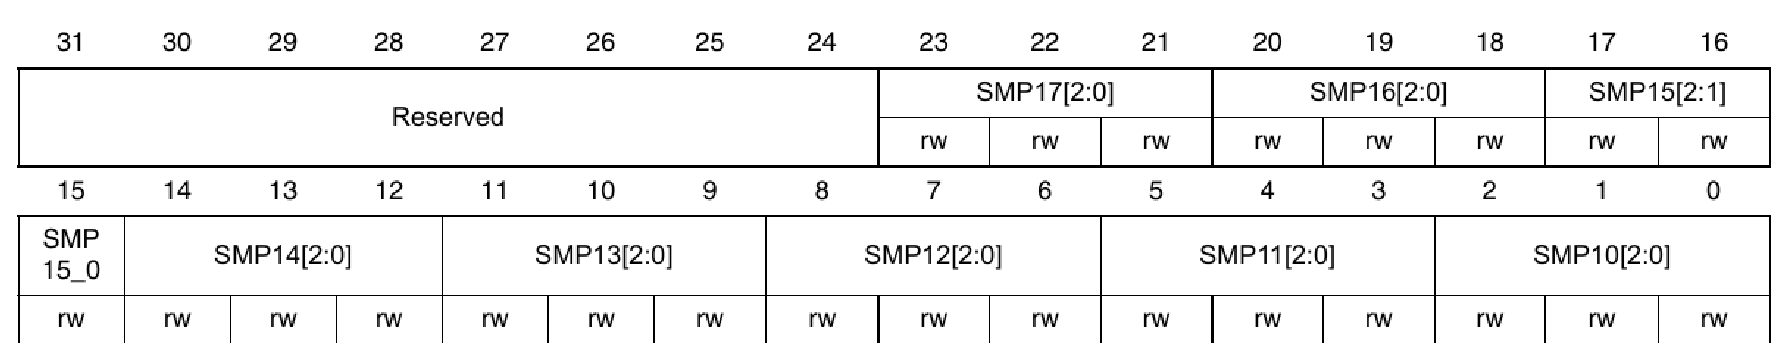
\includegraphics[width=\columnwidth]{./stm32/adc/figs/smpr1.eps}
\caption{SMPR1}
\label{fig:smpr1}
\end{figure}
%
\item What is the sampling time?
\\
\solution Since the sample time is 239.5 cycles and the ADC frequency is 14 MHz, 
\begin{equation}
T_{s} = 239.5 \times \frac{1}{14} \mu s = 17.1 \mu s 
\end{equation}
\item Explain the following instruction.
\begin{lstlisting}
ADC1->SQR3 |= ADC_SQR3_SQ1_4;
\end{lstlisting}

\solution ADC\_SQR3\_SQ1\_4 = 0x00000010.  This implies that SQ1=0b10000 in
the ADC regular sequence register 3 ($ADC1->SQR3$)shown in Fig. \ref{fig:sqr3}. Since SQ1=16,
this means that the ADC input in channel 16 will be the first in the queue
for conversion. 
%
\begin{figure}
\centering
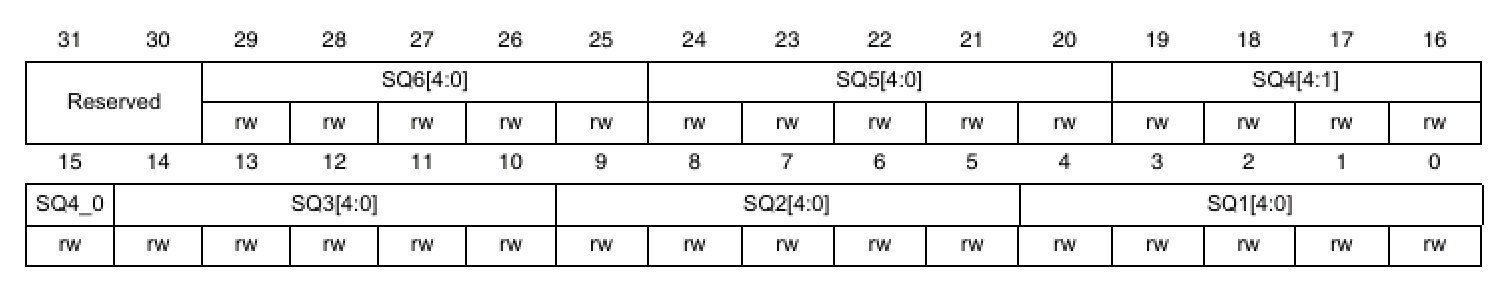
\includegraphics[width=\columnwidth]{./stm32/adc/figs/sqr3.eps}
\caption{SQR3}
\label{fig:sqr3}
\end{figure}
%
The ADC is capable of converting analog 16 inputs one after the other. 
The inputs are called {\em channels} and the sequence number corresponding 
to the channel
is decided
according to the 5 bit entry in SQ. 
\subsection{Measuring an Unkown Resistance}
\item Configure SQR3 so that the 9th channel for ADC1 is 2nd in sequence.
\\
\solution This implies that SQ2=1001.  Thus,
\begin{equation}
ADC1->SQR3 = 0x000000120
\end{equation}
\item List the various pin numbers corresponding to the different channels of the ADC.
\\
\solution See Fig. \ref{table:pin_channel}
\begin{table}[!ht]
\footnotesize
\input{./stm32/adc/figs/pin_channel.tex}
\caption{ADC Analog Input Pins}
\label{table:pin_channel}
\end{table}
\item Use the 9th channel of  ADC1 in SQ2 to measure 3.3V. 
\\
\solution Connect PB1 (Fig. \ref{table:pin_channel}) to 3.3 V of the STM 32 and execute the following
code.
\item Before flashing code to STM32 set the STM32 board to Programming mode as shown in Fig. \ref{fig:programming_mode}, then change the mode to Operating mode as shown in Fig. \ref{fig:programming_mode} after flashing the code inorder to run your program from main memory.
\begin{lstlisting}
cd /adc/3_3V.c
\end{lstlisting}
%\section{Project}
\item Measure an unkown resistance using the STM32 and display the result on the LCD.
\item Display the output of the internal temperature sensor as well the unknown resistance on the LCD.
\end{enumerate}

